\thispagestyle{empty}
%%!TEX encoding = UTF-8 Unicode
%%%\vspace*{1.2cm}
%%%%\begin{center}
%\noindent

%%\vskip30mm
%\vspace*{1cm}
%\begin{center}
%{\bf\Large 生物信息中的概率统计模型}
%
%邓明华,卜东波 编著
%\end{center}
%\vfill
%
%%\begin{flushright}
%\begin{center}
%{\bf 内部讲义}\\[2mm]
%{\bf $\bullet$北京$\bullet$ }
%\end{center}
%%%%%\vspace*{1cm} 


\begin{figure}[ht]
\centering
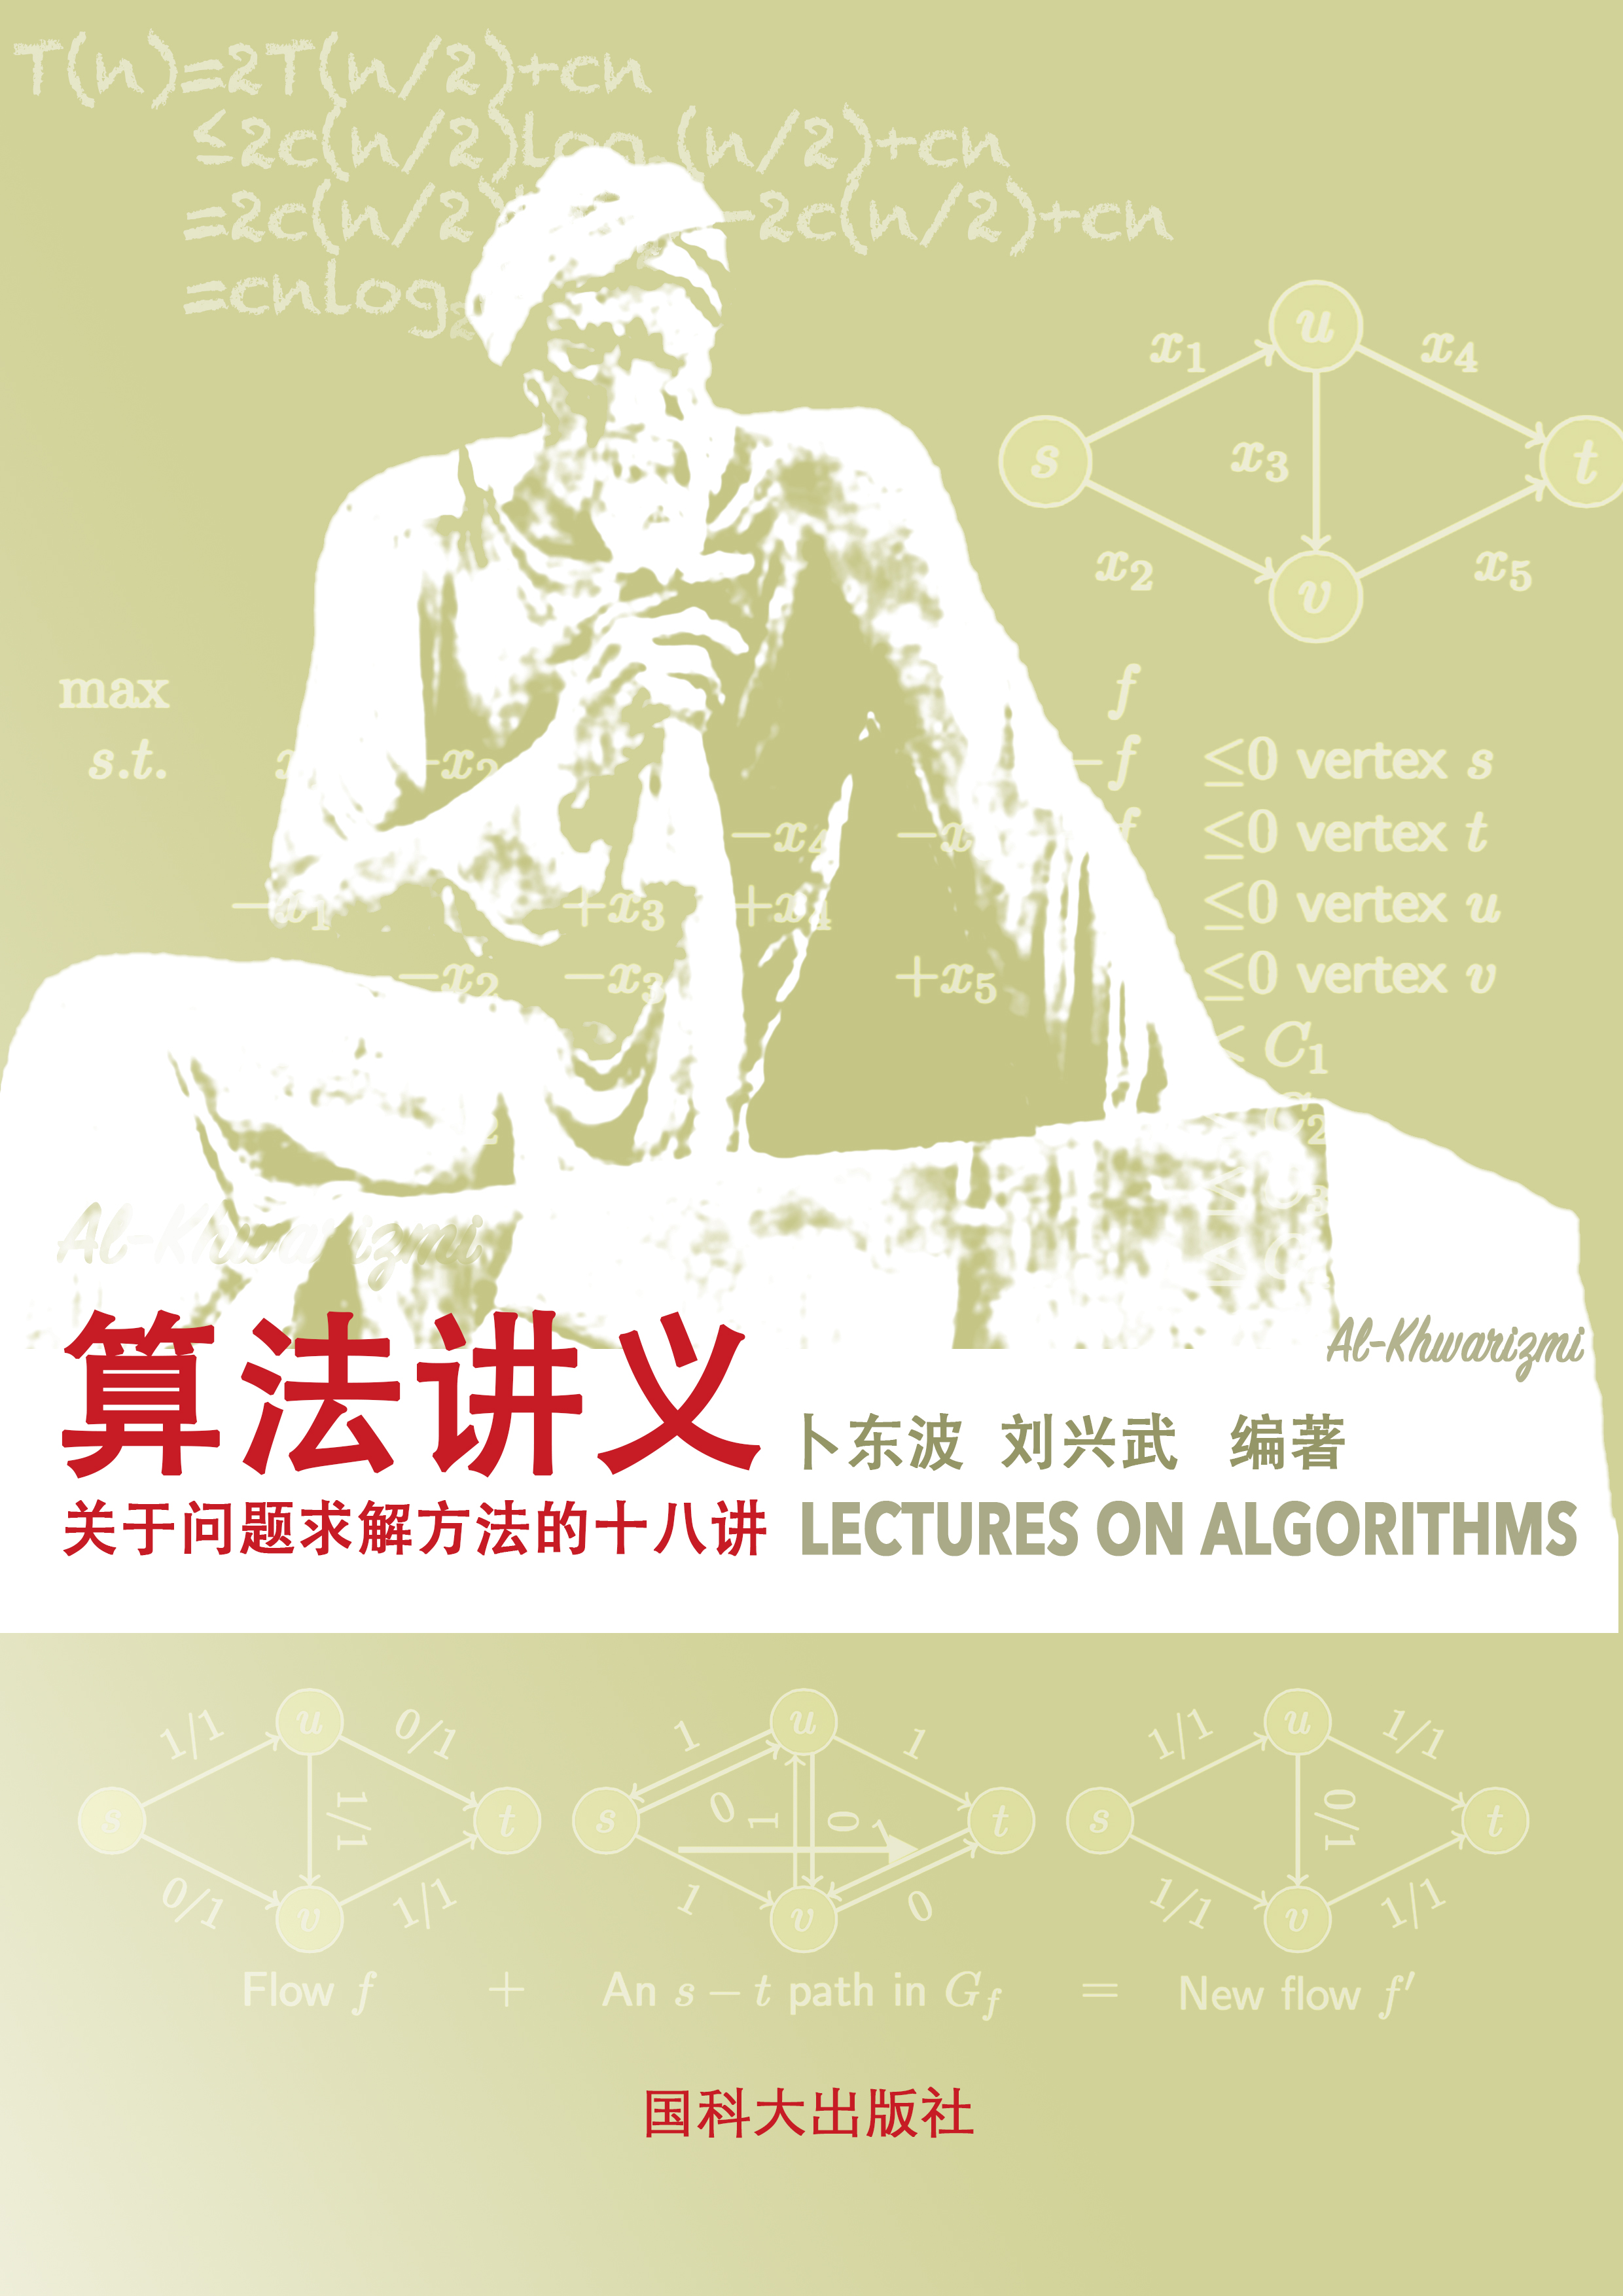
\includegraphics[width=1.1\textwidth] {BookCoverPage.png}
\end{figure}

\clearpage

%\chapter*{{\bf\large 内容简介}}
%%\thispagestyle{empty}
%%\end{center}
%%\vspace{6mm}
%\vskip -2mm
%
%本书是为大学非基础数学专业本科生编写的.它针对的对象是数学系非基础数学专业的学生,
%以及物理专业的学生.它的先修课程是数学分析或物理类的高等数学.
%全书共分6章,内容包括:集合,欧氏空间,Lebesgue测度,Lebesgue可测函数,
%测度空间,测度空间上的可测函数,测度空间上的积分,Lebesgue积分,$L^p$空间,
%$L^2$空间,卷积与Fourier变换,距离空间,Hilbert空间理论,
%Hilbert空间上的有界线性算子,Banach空间,Banach空间上的有界线
%算子,Banach空间上的连续线性泛函、共轭空间与共轭算子 ,Banach空间的
%收敛性与紧致性.
%
%本书在选材上注重了少而精,突出重点,尽可能地反映实变函数论与泛函分析中的
%核心内容;在内容的处理上, 本着由浅入深,循序渐进的原则;在介绍新理论的时候,
%尽可能地阐明它的背景,它与先前介绍过的的理论间的联系;在叙述表达上, 力求清晰易读,
%便于教学与自学.每节后配置了丰富的习题,其目的是为学生提供足够的练习,以便学生
%复习、巩固、理解和拓广所学知识.为了使书中的内容成为自封闭的,
%特编了四节附录附在正文之后,这样本书中所有的定理都给出严格的数学
%证明.书末附有部分习题的参考解答或提示.
%
%本书可作为综合大学、理工科大学、高等师范院校应用数学专业、计算数学专业、统计专业
%,以及物理专业本科生的教材或教学参考书, 也可供从事数学或物理研究
%的科技人员参考.
%
%
%\section*{{\bf\large 作者简介}}
%
%\noindent {\bf 邓明华} \quad 北京大学数学科学学院教授.
%1998年在北京大学数学科学学院获博士学位。美国南加州大学计算生物学中心博士后。
%主要研究方向是生物信息学。发表生物信息学论文50多篇,先后主持三项自然科学基金委面上项目和一项863项目,作为学术骨干参加三项973项目。
%
%\noindent {\bf 卜东波}\quad 中国科学院计算机技术研究所研究员.
%
% \clearpage

\chapter[{前言}]{前  言}
\vspace{2mm}
\setcounter{page}{1}

公元9世纪,波斯数学家Muhammad ibn Musa al-Khwarizmi写了一本名为{\it The Compendious Book on Calculation by Completion and Balancing}的书。

这本书记载了一些贸易、测量、遗产分配等方面的实际问题,以及从这些实际问题出发抽象建模而成的线性方程组和二次方程。更重要的是,这本书还介绍了求解上述方程的方法---这些方法具有清晰描述的步骤;任何人按步骤机械式地操作即可求解方程。这样的问题求解方法被称为``Algorithm",中文译作“算法”。Algorithm一词来源于Al-Khawarizmi名字的拉丁文译法,以表达人们对他的敬意。

无独有偶。中国古代的数学著作《九章算术》以及《九章算术注释》也是记载了许多实际问题以及相应的求解方法,甚至还提出“算”这一概念来表示“运算次数”,以比较不同求解方法的效率。中国古代数学重视解决来自现实生活的实际问题,而不像古希腊数学那样专注于证明定理。吴文俊先生称中国传统数学的特点是“高度的机械化和算法化”,并认为这一特点是和现代计算机科学密切相通的。

我们所写的这本讲义,是沿着“实际问题 $\Rightarrow$ 抽象出的数学问题 $\Rightarrow$ 算法设计”这条脉络总结我们的一些心得体会。如果说有一些特色的话,可能在于这本讲义不是简单地罗列现有的算法技术,而是试图强调“如何观察问题的结构”、强调“如何基于问题的结构进行算法设计”---求解问题的过程不应当只是逐个尝试各个算法技术或者纯粹依赖于灵感,而是应该依赖于我们对问题结构的认识;我们对问题结构认识得越深入,越有助于求解算法的设计。

这本讲义是沿着“首先观察问题结构、继而依据对问题结构的观察进行算法设计”这个问题求解思路来组织的。讲义分作三个大的部分,分别对应于不同的问题结构:$(i)$ 当我们观察到待求解的问题能够归约成规模较小的子问题时,就可以尝试“基于归约原理的算法设计”。这一类算法组成讲义的第一部分,包括“分而治之”算法(第2章)、动态规划算法(第3章)和贪心算法(第4章)。$(ii)$ 当我们观察到问题不太容易归约成规模较小的子问题、但是能够观察到可行解之间的变换关系时,就可以尝试“逐步改进”类算法设计策略。这一类算法组成讲义的第二部分,包括线性规划(第5章)及对偶理论(第6章)、网络流算法及其应用(第7, 8章)。$(iii)$ 难度是问题的本质属性。当我们观察到问题之间的归约关系、并进而证明了问题是NP-Hard(第9章),就意味着只有放松要求才能设计出高效的算法。这一类算法组成讲义的第三部分,包括只要求能够得到近似解的近似算法(第10章)、允许算法中存在随机化行为的随机算法(第11章),以及实用的启发式算法(第12章)。我们把问题求解思路的详细描述放在第1章,作为整个讲义的总纲。


我们在中国科学院大学的研究生班上多次讲授《算法设计与分析》课程,通常需要讲授一个学期、共十八次课。这本讲义是教学过程的自然结晶;我们加上副标题“关于问题求解方法的十八讲”,是想表达这本书和教学之间的紧密关系。在写作这本讲义时,我们想象中的读者是计算机专业的研究生或者高年级本科生;我们假定读者已经修习过《数据结构》和《计算机程序设计》,并熟练掌握至少一门计算机语言。


我在滑铁卢大学听过Timothy Chan讲授的算法课。在把复杂的算法讲得清楚明白这一点上,我从Timothy Chan那里领会到了很多。在写作风格方面,我偏爱于《费恩曼物理学讲义》的写法:要揭示复杂事物背后的直观思想,自然的笔触或许更有助于理解本质性的东西。这份讲义是采用这种写法的一次尝试---由中国科学院大学的同学们依据课堂录音整理成文;我们在此对乔扬、申世伟、邵益文、黄斌、闾泽军、乔晶、袁伟超、李飞、 孔鲁鹏、 吴步娇、 张敬玮、 罗纯龙、 曹晓然、 梁志鹏、 江涛等同学致以谢忱。

有很多同事、同学担任了《算法设计与分析》课程的助教,对这本讲义有直接的贡献。我们在此对林宇、袁雄鹰、邵明富、王超、张海仓、黄春林、李锦、黄琴、凌彬、王耀军、许情、张任玉、巩海娥、杨飞、王冰、高枫、李艳博、朱建伟、魏国正、鞠富松等同学表示诚挚的感谢---或许将他们列为本书的共同作者,更能彰显他们的贡献。

在讲授这门课程时,我们制作、使用了电子课件(包括幻灯片、算法演示,以及OJ编程题目);这些课件可以从{\tt http://bioinfo.ict.ac.cn/$\sim$dbu/AlgorithmCourses/ CS091M4041H/}下载。诸位读者在使用讲义和课件时所发现的错误,敬请发送至{\tt errata.lnoa@gmail.com}。

这本讲义的写作得到了李国杰、白硕、徐志伟等老师的鼓励。诸位师长奖掖后进,拳拳之心,使人难生懈怠之意。我们谨以这本小书回馈他们的希冀。


如何在讲清楚直观思想的同时又不丢失严谨性,是讲课和写作中最难把握的,也是最让我们困惑的。在这一点上,我们始终惴惴不安,只能静候读者的建议和指正。



%实变函数与泛函分析这两门课程是进入现代数学的门槛.我在60年代上大学时,实变函数
%已是数学系本科生高年级的必修课,但是泛函分析只是泛函专业学生的专业必修课. 当
%时的教材相当缺乏,主要的参考书是翻译的俄文教材或专著.
%
%1978年恢复高考以来,泛函分析课开始成为北京大学数学系本科生的一门必修课.这一方面因
%为这门课程的重要性,另一方面是因为在北京大学数学系这门课程已经十分成熟,完全有能力
%开好,而且相关教材的建设也取得很大成绩.周民强先生编著的$\langle\!\langle\,
%\mbox{实变函数}\,\rangle\!\rangle$,
%张恭庆与林源渠先生编著的$\langle\!\langle\,\mbox{泛函分析讲义}\,\rangle\!\rangle$
%上册分别于1985年和1987年出版.这两本教材编得非
%常成功,获得很高的评价. 此外,许多好的英文教材相继影印出版; 国内许多大学也出版了不少
%实变函数教材与泛函分析教材,有些是非常优秀的,有很大的影响. 总之实变函数与泛函分析这两
%门课程的建设相当成熟.那么为什么还要在北京大学开设称之为“实变函数与泛函分析”的一学期的课程呢?
%
%事实上教育事业一直处于不断的改革之中,北京大学数学系教学工作也在不断的改革中前进,关心和
%发展应用数学始终是改革的一个重要议题. 早在80年代北京大学数学系就增设了信息专
%业;1995年成立数学学院时又增设了金融数学专业. 根据“加强基础,淡化专业,因材施
%教,分流培养”的方针,本科生教育增加了计算机方面的课程,还添设了数学模型课等.由
%于学制是四年,尽管泛函分析课仍是基础数学、计算数学和概率论的专业必修课,但是一
%些应用学科的专业已经不可能再安排一学期的泛函分析课.然而无论是金融数学还是
%信息学科,乃至物理学科各专业的本科生应当有一些泛函分析的训练, 这是大家的共识.
%于是就提出开设一学期的实变函数与泛函分析课的要求. 应领导的安排我在两年前开始
%考虑设计这门课.
%
%实变函数与泛函分析已经是相当成熟的课程,其内容已经高度浓缩,它们所涵盖的理论
%和内容都是十分基本的或者是十分重要的.现在有许多优秀的中文教材和外文教材,要
%编写有新意的教材无疑是一桩难题,更何况要将一学年的课程压缩成一学期的课程,
%这样的教材就更难编写了. 于是我考察对比了十多本优秀教材,反复思考应当保留什么?也就是应
%当舍去什么?结果发现这样根本无法进行下去,因为许多精彩的理论同时也是重要的理
%论都很难将其砍掉. 于是我决定改变思路,先确定这门课的主线. 这门课程的
%一条线是:欧氏空间\!\!--\!--\!Lebesgue平方可积函数空间\!\!--\!--\,Hilbert空间;与此同时还有平行的
%另一条线:欧氏空间\!\!--\!--\,$p$次Lebesgue可积函数空间\!\!--\!--\,Banach空间,前者是后者的特例.
%这两条线可以有合有分,有机地揉在一起而组成这门课的主线. 以主线为纲,纲举目张
%,就可以添枝加叶了.
%
%作者编写这本教材,力求通过一学期课程的讲授,使学生了解Banach空间中拓扑现象的描述和它
%代表的内涵,了解无穷维Banach空间与有穷维欧氏空间的对比及其异同,并使学生了解
%$p$次Lebesgue可积函数空间的理论即是理解以上思想的纽结和穴位. 作者在组织内容方面
%力求做到由浅入深,由点到面,循序渐进的原则;在叙述表达上力求清晰易读,便于教学和
%阅读.为了使得教材精练,还将一些重要定理的证明放在书末的附录里以便读者自学.
%尽管做了许多努力正文部分仍有300余页,内容似乎还是多了一些,建议教员在讲授时不要
%每个定理都证明,应当选取适当材料留给学生阅读,比如抽象测度空间理论,包括测度空间上的
%可测函数、可积函数等,以培养学生的自学能力. 对于教学而言,
%这是建设一门新课程;对于作者而言,这是编写新讲义,是初次的尝试, 疏漏与不足之处在所难
%免,热诚欢迎读者批评指正.
%
%本书的写作得到北京大学数学科学学院和北京大学出版社的大力支持,作者对他们表示衷心的感谢.
%本书的写作还得到北京市高等教育精品教材建设项目的资助,作者对此表示衷心的感谢.本书
%的责任编辑邱淑清女士是我的师长.她为本书的出版倾注了很多心血,作了大量辛勤的工作.作者对她
%表示衷心的感谢.



\vskip10mm

\mbox{}\hfill
\shortstack[c]{卜东波、张家琳 \\ [2mm] 2018年于中科院计算所、中国科学院大学}\mbox{}\hfill
\clearpage

%\mbox{}
%\thispagestyle{empty}
%\clearpage

